\section{Randomized Algorithm with Attempts}

The second algorithm, \textit{randomized\_fpt\_attempts}, was conceived to improve the solution-finding strategy utilized by the first algorithm. In particular, this algorithm was designed to mitigate the first algorithm's shortfall in discovering a sufficient number of viable solutions by performing multiple attempts and ensuring each set of vertices selected to form a potential vertex cover was unique, expanding the search space without revisiting the previously tested configurations.
Although this proved to be more time-consuming, as explained further ahead, it did provide more solutions.

\subsection{Pseudocode}
\begin{algorithm}
\caption{Randomized FPT Attempts}
\begin{algorithmic}[1]
\Procedure{randomized\_fpt\_attempts}{$graph, k, max\_attempts = 10000$}
\State $vertex\_cover \gets \text{set}()$
\State $tested\_combinations \gets \text{set}()$
\For{$\_ \in \text{range}(max\_attempts)$}
\State $vertex\_cover \gets \text{set}()$
\State $remaining\_graph \gets graph.copy()$
\State $added\_vertices \gets \text{set}()$
\While{$\text{len}(vertex\_cover) < k$}
\If{$\text{len}(remaining\_graph.edges()) = 0$}
\State \textbf{break}
\EndIf
\State $edge \gets \text{random.choice}(\text{list}(remaining\_graph.edges()))$
\State $vertex \gets \text{random.choice}(edge)$
\If{$vertex \in added\_vertices$}
\State \textbf{continue}
\EndIf
\State $vertex\_cover.add(vertex)$
\State $added\_vertices.add(vertex)$
\State $edges\_to\_remove \gets [e \text{ for } e \text{ in } remaining\_graph.edges(vertex)]$
\State $remaining\_graph.remove\_edges\_from

(edges\_to\_remove)$


\EndWhile
\State $combination \gets \text{frozenset}(vertex\_cover)$
\If{$combination \in tested\_combinations$}
\State \textbf{continue}
\EndIf
\State $tested\_combinations.add(combination)$
\If{$\text{is\_vertex\_cover}(graph, vertex\_cover)$}
\State \textbf{break}
\EndIf
\EndFor
\If{$\text{len}(remaining\_graph.edges()) = 0$ \textbf{and} $\text{len}(vertex\_cover) = k$}
\State \Return $vertex\_cover$
\Else
\State \Return $\text{None}$
\EndIf
\EndProcedure
\end{algorithmic}
\end{algorithm}

\subsection{Formal Analysis}
The time complexity of the \textit{randomized\_fpt\_attempts} algorithm is influenced by introducing a maximum number of attempts to find a vertex cover. Each attempt randomly selects edges and vertices and removes all incident edges to the selected vertex, similar to the first algorithm.

In terms of complexity analysis:
\begin{itemize}
  \item \textbf{Best Case:} The best case occurs when a vertex cover of size \(k\) is found without reaching the maximum number of attempts and without revisiting previously tested configurations. This scenario benefits from the non-redundant solution space exploration and can have a complexity better than \(O(k \cdot m)\). However, this is highly dependent on the randomness of the selection process and the graph structure.
  
  \item \textbf{Average Case:} The average case considers the potential revisiting of certain vertex sets due to random selection despite the attempt to avoid redundancy. This could result in an average time complexity still approximately \(O(k \cdot m)\), with the added overhead of managing the tested combinations.

  \item \textbf{Worst Case:} The worst-case scenario occurs when the maximum number of attempts is reached without finding a satisfactory vertex cover. In this case, the algorithm's complexity is affected by the cap on attempts and the overhead of tracking tested combinations, potentially leading to a complexity of \(O(max\_attempts \cdot k \cdot m)\), assuming the worst case happens at the last attempt.
\end{itemize}

\subsection{Experimental Analysis}
To empirically assess the algorithm's performance, it was tested on randomly generated graphs with varying numbers of vertices and edges. The parameters were:

\begin{itemize}
    \item \(n\) (number of vertices) Range: From 4 to 256, to cover a broad spectrum of graph sizes.
    \item \(m\) (number of edges) Proportions: Fixed percentages of the maximum possible number of edges, specifically \{0.125, 0.25, 0.5, 0.75\} of the maximum.
    \item \(k\) (vertex cover size) Proportions: Relative to the number of vertices, with proportions \{0.125, 0.25, 0.5, 0.75\}.
\end{itemize}

Two metrics were evaluated:\begin{enumerate}
    \item Number of Basic Operations: Operations for each random selection of edges and vertices, and for edge removals.
    \item Number of Solutions Tested: Total number of vertex cover sets attempted until the algorithm terminates.
\end{enumerate}

For the analysis, we focused on the first iteration, as we did in the \textit{randomized\_fpt} algorithm analysis.

\subsubsection{Analysis of Operations}
The number of operations indicates the algorithm's computational effort for each vertex cover size and edge density. As evidenced by Figures \ref{fig:atmpts_num_operations_k12_5} and \ref{atmpts_num_operations_k75}, the algorithm demonstrates a growth pattern in the number of operations, which appears to be influenced by the edge density. Higher edge densities correspond to more operations, suggesting a non-linear relationship between the edge density and computational complexity.

\begin{figure}[h]
\centering
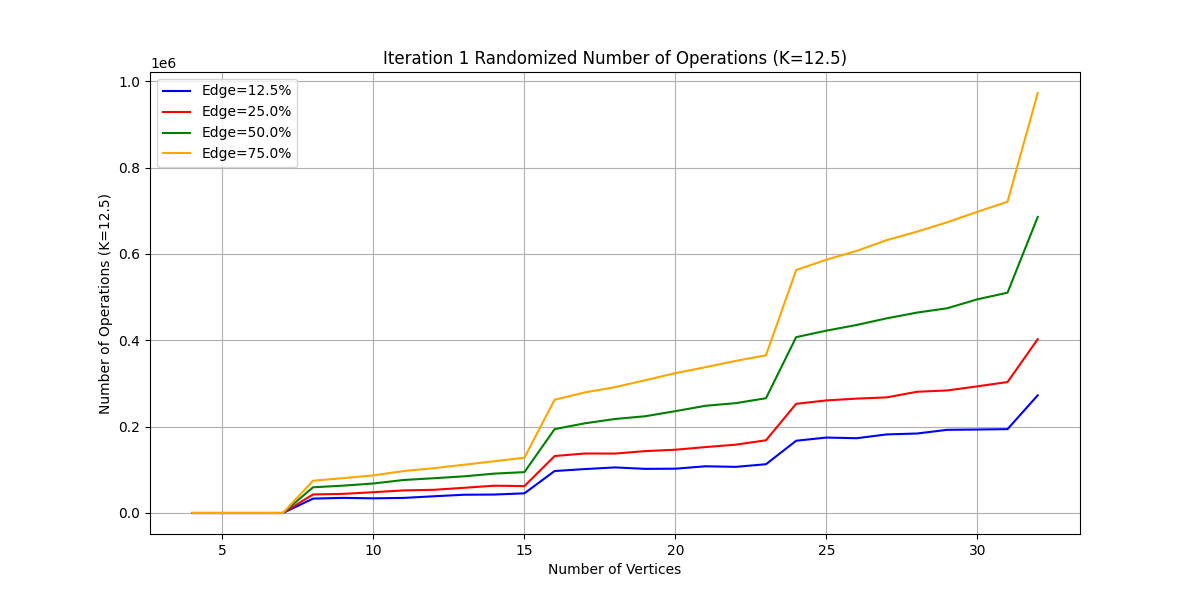
\includegraphics[width=0.5\textwidth]{FPT_attempts/Number of Operations (K=12.5).png}
\caption{FPT Attempts \(|\) Number of operations for \( K=12.5 \).}
\label{fig:atmpts_num_operations_k12_5}
\end{figure}

\begin{figure}[h]
\centering
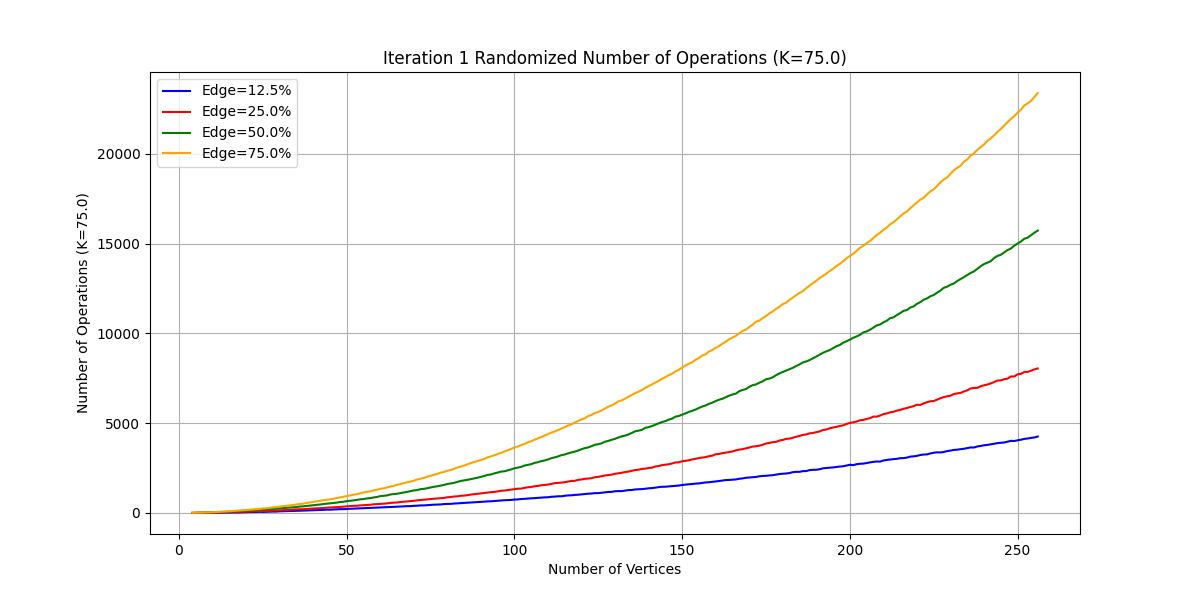
\includegraphics[width=0.5\textwidth]{FPT/Number of Operations (K=75.0).png}
\caption{FPT Attempts \(|\) Number of operations for \( K=75.0 \).}
\label{fig:atmpts_num_operations_k75}
\end{figure}

\subsubsection{Analysis of Solutions Tested}
The number of solutions tested reflects the algorithm's exploration depth in the search for a valid vertex cover. Figures \ref{fig:atmpts_sol_tested_k12_5} and \ref{fig:atmpts_sol_tested_k75} display the total number of vertex cover sets attempted. The variability observed, particularly the spikes in the number of solutions tested, suggests instances where the algorithm may be inefficiently cycling through combinations, especially at higher edge densities.

\begin{figure}[h]
\centering
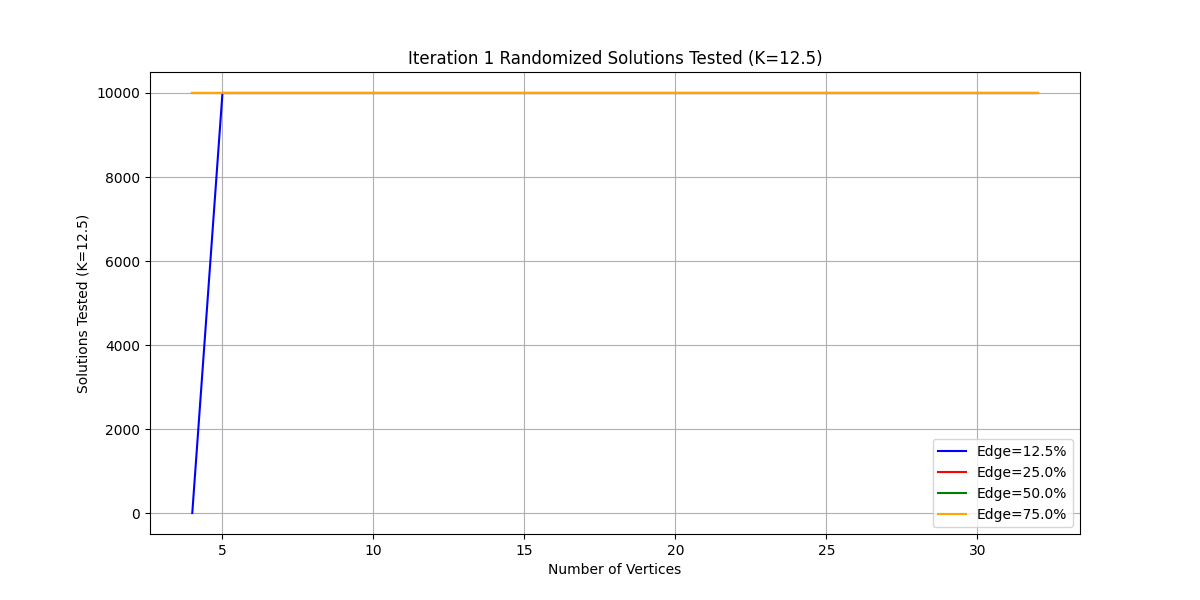
\includegraphics[width=0.5\textwidth]{FPT_attempts/Solutions Tested (K=12.5).png}
\caption{FPT Attempts \(|\) Number of solutions tested for \( K=12.5 \).}
\label{fig:atmpts_sol_tested_k12_5}
\end{figure}

\begin{figure}[h]
\centering
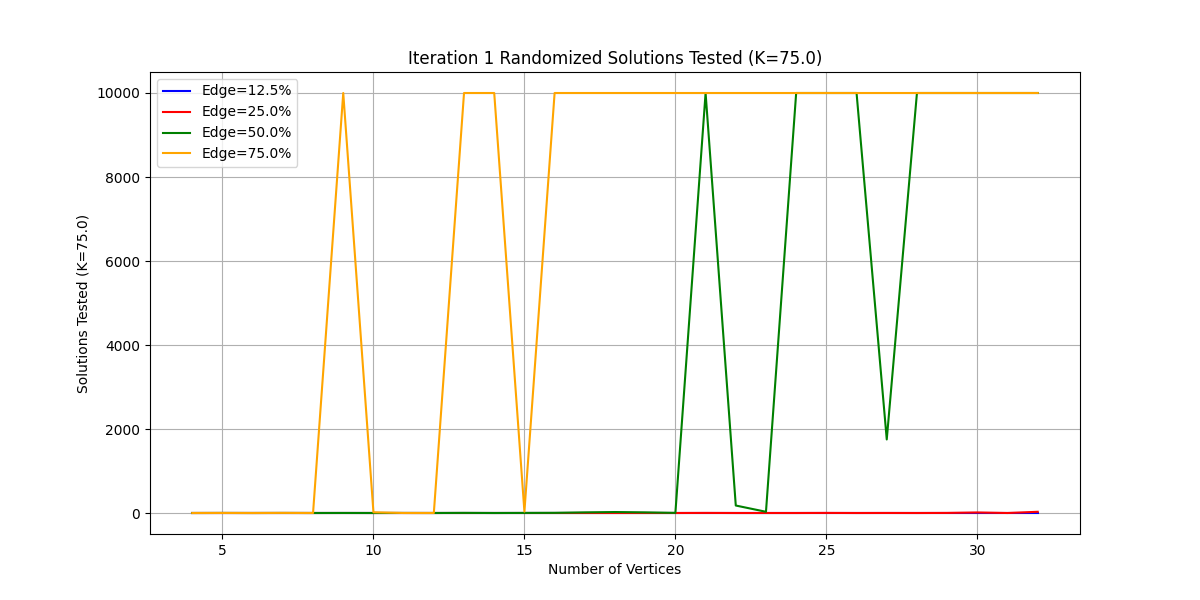
\includegraphics[width=0.5\textwidth]{FPT_attempts/Solutions Tested (K=75.0).png}
\caption{FPT Attempts \(|\) Number of solutions tested for \( K=75.0 \).}
\label{fig:atmpts_sol_tested_k75}
\end{figure}

\subsubsection{Conclusions from the Experimental Analysis}
The single iteration analysis shows that the \textit{randomized\_fpt\_attempts} algorithm exhibits considerable variability in its performance, which is heavily influenced by the graph's edge density. While the algorithm can explore a wide range of solutions, the spikes in the number of solutions tested indicate potential inefficiencies. The increased number of operations with higher edge densities also suggests that the algorithm's computational load may grow significantly with more complex graphs. These insights underscore the necessity for further optimization to improve the algorithm's consistency and efficiency.


\subsection{Performance of the Second Algorithm}
The algorithm introduces a cap of \(10000\) on the number of solution attempts, aiming to overcome the limitations of the first algorithm in finding sufficient feasible solutions. By tracking previously tested vertex combinations, the algorithm avoids redundant computations. However, the performance, as demonstrated in Figures \ref{fig:atmpts_sol_tested_k12_5} and \ref{fig:atmpts_sol_tested_k75}, showed substantial variability in the number of solutions tested, which sometimes led to high peaks. These peaks indicate inefficiency and a potential oversimplification in the solution space exploration.

\subsection{Comparative Analysis with the First Algorithm}
Compared to the first algorithm, the second algorithm's objective was to enrich the set of solutions rather than minimize the computational time. Despite this, the second algorithm did not consistently yield a broader spectrum of solutions. The erratic nature of the results, especially in the number of solutions tested, highlights the challenges in balancing exploration depth with computational efficiency. In contrast, despite its limitations in discovering diverse solutions, the first algorithm exhibited a more stable and predictable pattern.

The findings suggest that the second algorithm's strategy of limiting attempts may not be sufficient to address the complexities of the vertex cover problem. Future enhancements could focus on more sophisticated methods of solution space exploration to reliably extend the range of solutions discovered.


